% =========================================================================
% 《高中數學實驗教材》第二冊（高一下） 
% 第三章 實數系及其基本性質
% =========================================================================

\section{實數系及其基本性質}\label{sec:b2_ch3}

在第一冊的第三章中，我們會簡略地說明了幾個數系間的包含關係\phantomsection\label{note:b2-ch3-ceng}：
\[
\mathbb{R} \supseteq \mathbb{Q} \supseteq \mathbb{Z} \supseteq \mathbb{N} \quad \text{（註\footnote{集合包含關係的符號 $\supseteq$ 也可省略下面的一橫，寫為 $\supset$，都表示包含或相等. 當我們要指出包含而不相等的關係時，可以採用符號 $\supsetneq$，例如上述各數系間的包含關係，就可以更確實地寫為 $\mathbb{R} \supsetneq \mathbb{Q} \supsetneq \mathbb{Z} \supsetneq \mathbb{N}$.}）}
\]
\[
\text{（實數系）}\quad\text{（有理數系）}\quad\text{（整數系）}\quad\text{（自然數系）}
\]
並且以自然數系的基本性質為出發點，逐步經由上述關係去討論整數系及有理數系的基本性質. 本章將進一步用上一章所討論的極限概念，利用有理數系與實數系間的包含關係去瞭解實數系的性質.

\subsection{有理數系與實數系}\label{sec:b2_3-1}

\subsubsection*{1-1 我們先用上一章 § 2 中所介紹的直線坐標系來圖解說明有理數系與實數系間的關係.}

\begin{center}
\begin{tikzpicture}[x=1.05cm, y=1.1cm]
    % Main coordinate axis
    \draw[thick, <->] (-5.6, 0) -- (6.6, 0);
    
    % Integer ticks and labels
    \foreach \x in {-5,-4,-3,-2,-1,0,1,2,3,4,5,6} {
        \draw[thick] (\x, 0.15) -- (\x, -0.15);
        \node[font=\footnotesize] at (\x, 0.35) {$\x$};
    }
    
    % Halves above the line
    \foreach \x/\num in {-4.5/-9, -3.5/-7, -2.5/-5, -1.5/-3, -0.5/-1, 0.5/1, 1.5/3, 2.5/5, 3.5/7, 4.5/9, 5.5/11} {
        \draw[thin] (\x, 0.1) -- (\x, 0);
        \node[font=\scriptsize] at (\x, 0.75) {$\frac{\num}{2}$};
    }
    
    % Thirds below the line
    \foreach \x/\num in {-4.667/-14, -4.333/-13, -3.667/-11, -3.333/-10, -2.667/-8, -2.333/-7, -1.667/-5, -1.333/-4, -0.667/-2, -0.333/-1, 0.333/1, 0.667/2, 1.333/4, 1.667/5, 2.333/7, 2.667/8, 3.333/10, 3.667/11, 4.333/13, 4.667/14, 5.333/16, 5.667/17} {
        \draw[thin] (\x, -0.1) -- (\x, 0);
        \node[font=\scriptsize] at (\x, -0.65) {$\frac{\num}{3}$};
    }
    
    % Unit length bracket
    \draw[|-|, thin] (0, -1.25) -- (1, -1.25);
    \node[below, font=\footnotesize] at (0.5, -1.25) {（單位長）};
\end{tikzpicture}
\end{center}

在上面的坐標系中，所有以整數為坐標的點，在直線上成一均勻分布的點集，其相鄰兩點間的距離都是 1 單位. 同樣的，所有坐標是 $\frac{n}{2}\;(n=0, \pm 1, \pm 2, \dots\dots)$ 的點，在直線上成一均勻分布的點集，其相鄰兩點間的距離都是 $\frac{1}{2}$ 單位，以此類推，設 $k$ 為一指定自然數，則所有坐標是 $\frac{n}{k};\; n\in\mathbb{Z}$ 的點在直線上成一均勻分布的點集，其相鄰兩點間的距離為 $\frac{1}{k}$ 單位. 所以當 $k$ 逐漸增大時，上述點集就愈來愈密.（亦即相鄰兩點之間的距離 $\frac{1}{k}$ 遞減而趨於 0 為「極限」.）所以直線上任何一個線段都包含 $\frac{n}{k}$ 這樣的點.

在直線上，所有坐標是有理數的點所成的集合，顯然就是所有上面所列舉的點集，這點集裡的元素稱為有理數點. 在直線上任何一段很短的線段中，都有坐標是有理數的點，也可以說，有理數點是無「孔」不入的. 這就是有理數點集的稠密性，換句話說，有理數點是在直線上到處稠密的.

但是這個現象並不表示有理數點就可以“填滿”整個直線. 事實上，從下面簡單的例子可以看出直線上還有一些點是不能用有理數來表示的（也就是說，這種點的坐標不是有理數）.

\subsubsection*{1-2 由畢氏定理，我們得知下列三個直角三角形的斜邊長分別是 $\sqrt{2}$ 單位、$\sqrt{3}$ 單位及 $\sqrt{5}$ 單位.}

\begin{center}
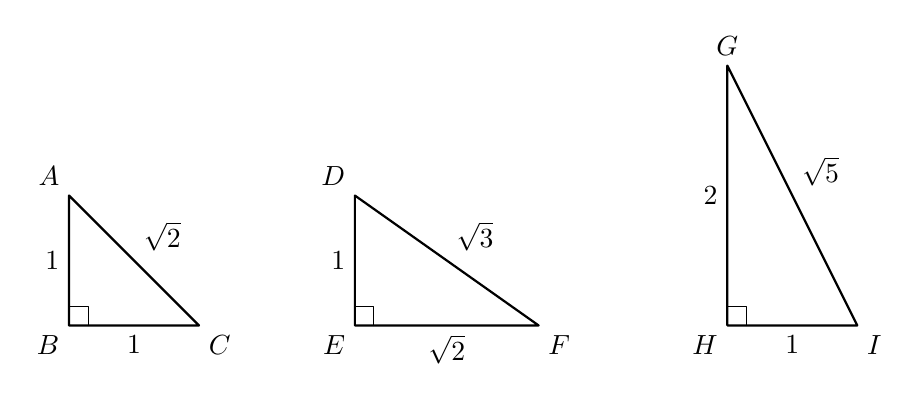
\begin{tikzpicture}[scale=1.1, line cap=round, line join=round]
    % Triangle 1: ABC
    \coordinate (B) at (0, 0);
    \coordinate (C) at (1.5, 0);
    \coordinate (A) at (0, 1.5);
    \draw[thick] (A) -- (B) -- (C) -- cycle;
    \draw (0, 0.22) -- (0.22, 0.22) -- (0.22, 0);
    \node[above left] at (A) {$A$};
    \node[below left] at (B) {$B$};
    \node[below right] at (C) {$C$};
    \node[left] at (0, 0.75) {$1$};
    \node[below] at (0.75, 0) {$1$};
    \node[above right] at (0.75, 0.75) {$\sqrt{2}$};

    % Triangle 2: DEF
    \begin{scope}[xshift=3.3cm]
    \coordinate (E) at (0, 0);
    \coordinate (F) at ({1.5*1.4142}, 0);
    \coordinate (D) at (0, 1.5);
    \draw[thick] (D) -- (E) -- (F) -- cycle;
    \draw (0, 0.22) -- (0.22, 0.22) -- (0.22, 0);
    \node[above left] at (D) {$D$};
    \node[below left] at (E) {$E$};
    \node[below right] at (F) {$F$};
    \node[left] at (0, 0.75) {$1$};
    \node[below] at ({0.75*1.4142}, 0) {$\sqrt{2}$};
    \node[above right] at ({0.75*1.4142}, 0.75) {$\sqrt{3}$};
    \end{scope}

    % Triangle 3: GHI
    \begin{scope}[xshift=7.6cm]
    \coordinate (H) at (0, 0);
    \coordinate (I) at (1.5, 0);
    \coordinate (G) at (0, 3.0);
    \draw[thick] (G) -- (H) -- (I) -- cycle;
    \draw (0, 0.22) -- (0.22, 0.22) -- (0.22, 0);
    \node[above] at (G) {$G$};
    \node[below left] at (H) {$H$};
    \node[below right] at (I) {$I$};
    \node[left] at (0, 1.5) {$2$};
    \node[below] at (0.75, 0) {$1$};
    \node[above right] at (0.75, 1.5) {$\sqrt{5}$};
    \end{scope}
\end{tikzpicture}
\end{center}

\begin{align*}
\overline{AC}^2 &= \overline{AB}^2 + \overline{BC}^2 = 1^2 + 1^2 = 2, \\
\overline{DF}^2 &= \overline{DE}^2 + \overline{EF}^2 = 1^2 + (\sqrt{2})^2 = 3, \\
\overline{GI}^2 &= \overline{GH}^2 + \overline{HI}^2 = 2^2 + 1^2 = 5.
\end{align*}
但是由第一冊第七章 § 2 中推論 2 可證 $x^2-2=0, x^2-3=0$ 及 $x^2-5=0$ 沒有「有理根」. 所以 $\sqrt{2}, \sqrt{3}$ 及 $\sqrt{5}$ 都是不屬於有理數系的實數. 因此，當我們在直線上取一點 $x$ 使得 $\overline{Ox}=\overline{AC}$（或 $\overline{DF}$ 或 $\overline{GI}$）就可以看出 $x$ 不是有理數點.

不屬於有理數系的實數有很多很多，上面三個數不過是隨便舉的幾個簡單的例子而已.

\subsubsection*{1-3 總結本節的討論，我們把有理數系與實數系間的關係扼要的敘述如下：}

\begin{enumerate}[(i)]
    \item 有理數系是實數系中一個到處稠密的子集. 但是實數系除了有理數之外，還包含有許多許多不是有理數的數，通常（相對地）叫做無理數.（註\footnote{中文的「有理數」譯自「rational number」；「無理數」譯自「irrational number」. 其實 rational 是 ratio 的形容詞，所以應該譯成「比數」和「非比數」才對. 但是很不幸的當年翻譯者把上述「rational」及「irrational」誤譯成「有理」及「無理」. 如今以訛傳訛，沿用至今. 現在似乎不更正反而比更正它還「有理」些. 特此註明.}）
    \item 因為有理數系在實數系中到處稠密，所以我們可以用有理數的「數列」去「逼近」任何一個給定實數. 換句話說，任何一個給定實數都是某一適當的有理數數列的極限.
\end{enumerate}
我們將在下一節中，用實例詳細解釋第 (ii) 點.

\subsection*{習題 3-1}

\begin{enumerate}
    \item 寫出 $\sqrt{2+\sqrt{2}}$ 和 $\sqrt{2-\sqrt{2}}$ 都能滿足的整數係數多項式方程式.
    \item 分別寫出下列各數能滿足的整數係數多項式方程式：
    \begin{enumerate}[(i)]
        \item $\sqrt{2+\sqrt{3}}$.
        \item $\sqrt[3]{3+\sqrt{3}}$.
        \item $\sqrt[3]{3+\sqrt{3+\sqrt{2}}}$.
        \item $\sqrt{2+\sqrt{3+\sqrt{2}}}$.
    \end{enumerate}
    \item 利用圓規和直尺作出長度如下的各線段：
    \begin{enumerate}[(i)]
        \item $\sqrt{2+\sqrt{2}}$.
        \item $\sqrt{3+\sqrt{2+\sqrt{2}}}$.
        \item $\sqrt{5-\sqrt{3}}$.
        \item $\sqrt{\sqrt{6}-1}$.
    \end{enumerate}
    \item 證明在兩個不同的有理數 $a, b$ 之間，存在無限多有理數 $x$，使得 $a < x < y$\phantomsection\label{note:b2-ch3-ex3-1-q4-xy}.
    \item 請找出下列“證明”中的錯誤：$a \neq b$，令 $c = \frac{a+b}{2}$，\\
    所以 $2c = a+b$, $2c(a-b) = (a+b)(a-b) = a^2-b^2$,\\
    $\therefore b^2-2bc = a^2-2ac$. 兩邊各加上 $c^2$ 得
    \[
    (b-c)^2 = b^2-2bc+c^2 = a^2-2ac+c^2 = (a-c)^2.
    \]
    所以 $b-c = a-c$，所以 $b=a$.
\end{enumerate}

\subsection{二分逼近法}\label{sec:b2_3-2}

在引言裡我們已經很具體地指出實數系是由度量所產生的數系，其中包含的數比有理數系包含的數要多得多. 不能用有理數來表示的長度，是不是可以用有理數來表示它的近似值呢？這就是 § 1-3 提出的，也就是這一節所要詳細討論的.

\subsubsection*{2-1 事實上，以十進位 (decimal number system) 數字法寫成的有限位數小數已不敷表示所有的有理數. 在第二章，§ 6 的例子中，我們已討論了如何以有限小數去逼近 $\frac{2}{3}$，就是十等分逼近法. 當我們用 3 去除 2，即逐步得到下列諸式：}

\begin{align}
2 = 0.6 \times 3 + 0.2 &\implies 0.6 < \frac{2}{3} < 0.7, \label{eq:b2-ch3-div-1} \\
2 = 0.66 \times 3 + 0.02 &\implies 0.66 < \frac{2}{3} < 0.67, \label{eq:b2-ch3-div-2} \\
&\ \ \cdots\cdots\cdots\cdots\cdots\cdots\cdots\cdots \notag \\
2 = 0.\underbrace{66\dots 66}_{n} \times 3 + 0.\underbrace{00\dots 0}_{n-1}2 &\implies 0.\underbrace{66\dots 66}_{n} < \frac{2}{3} < 0.\underbrace{66\dots 67}_{n}. \tag{$n$}\label{eq:b2-ch3-div-n}
\end{align}

以上諸式可用直線坐標系加以圖解說明如下：

\begin{center}
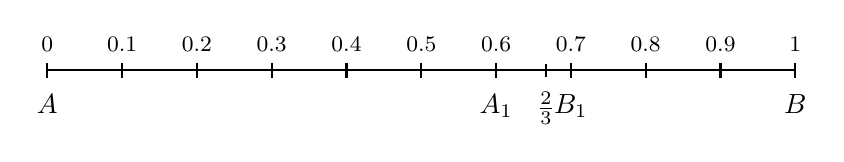
\begin{tikzpicture}[x=9.5cm, y=1cm]
    \draw[thick] (0, 0) -- (1, 0);
    \foreach \x in {0, 0.1, 0.2, 0.3, 0.4, 0.5, 0.6, 0.7, 0.8, 0.9, 1.0} {
        \draw[thick] (\x, 0.1) -- (\x, -0.1);
    }
    \node[above, font=\footnotesize] at (0, 0.12) {$0$};
    \node[above, font=\footnotesize] at (0.1, 0.12) {$0.1$};
    \node[above, font=\footnotesize] at (0.2, 0.12) {$0.2$};
    \node[above, font=\footnotesize] at (0.3, 0.12) {$0.3$};
    \node[above, font=\footnotesize] at (0.4, 0.12) {$0.4$};
    \node[above, font=\footnotesize] at (0.5, 0.12) {$0.5$};
    \node[above, font=\footnotesize] at (0.6, 0.12) {$0.6$};
    \node[above, font=\footnotesize] at (0.7, 0.12) {$0.7$};
    \node[above, font=\footnotesize] at (0.8, 0.12) {$0.8$};
    \node[above, font=\footnotesize] at (0.9, 0.12) {$0.9$};
    \node[above, font=\footnotesize] at (1.0, 0.12) {$1$};

    \node[below, font=\normalsize] at (0, -0.18) {$A$};
    \node[below, font=\normalsize] at (0.6, -0.18) {$A_1$};
    \draw[thin] (0.6667, 0.08) -- (0.6667, -0.08);
    \node[below, font=\normalsize] at (0.6667, -0.15) {$\frac{2}{3}$};
    \node[below, font=\normalsize] at (0.7, -0.18) {$B_1$};
    \node[below, font=\normalsize] at (1.0, -0.18) {$B$};
\end{tikzpicture}
\end{center}

\eqref{eq:b2-ch3-div-1} 式在上述坐標系中的意義是：\\
當我們把線段 $\overline{AB}=[0, 1]$ 等分為 10 段，$\frac{2}{3}$ 位於其第七段 $\overline{A_1 B_1} = [0.6, 0.7]$ 中.

\eqref{eq:b2-ch3-div-2} 式在上述坐標系中的意義是：\\
當我們把線段 $\overline{A_1 B_1}=[0.6, 0.7]$ 再等分為 10 段後，$\frac{2}{3}$ 位於線段 $\overline{A_2 B_2} = [0.66, 0.67]$ 中.

以此類推，\eqref{eq:b2-ch3-div-n} 式的意義是：\\
當我們把線段 $\overline{A_{n-1} B_{n-1}} = [0.\underbrace{66\dots\dots 66}_{n-1}, 0.\underbrace{66\dots\dots 67}_{n-1}]$ 再等分為 10 段時，$\frac{2}{3}$ 位於線段 $\overline{A_n B_n} = [0.\underbrace{66\dots\dots 66}_{n}, 0.\underbrace{66\dots\dots 67}_{n}]$ 中.

依樣畫葫蘆，對任意實數 $\xi$ 我們亦可以用「有限小數」去逼近它. 假設 $\xi$ 位於線段 $\overline{A_0 B_0}=[k, k+1]$ 內，（亦即 $(k < \xi < k+1)$.）逼近方法是：將線段 $\overline{A_0 B_0}$ 逐次用十等分法求出線段 $\overline{A_1 B_1}, \overline{A_2 B_2}, \dots\dots, \overline{A_n B_n}, \dots\dots$ 滿足下列性質：
\begin{enumerate}[(i)]
    \item $\overline{A_0 B_0} \supseteq \overline{A_1 B_1} \supseteq \overline{A_2 B_2} \supseteq \dots\dots \supseteq \overline{A_n B_n} \supseteq \dots\dots \supseteq \{\xi\}$.
    \item $\overline{A_n B_n} = \frac{1}{10^n} = \frac{1}{10}\overline{A_{n-1} B_{n-1}}$.（線段長）
    \item 如果以 $a_n, b_n$ 表示 $A_n, B_n$ 的坐標，顯然 $a_n, b_n$ 是 $n$ 位小數，而且 $b_n - a_n = \overline{A_n B_n} = \frac{1}{10^n}$.
    \[
    k = a_0 \le a_1 \le a_2 \le \cdots \le a_n \le \cdots \le \xi \le \cdots \le b_n \le \cdots \le b_2 \le b_1 \le b_0 = k+1.
    \]
    \item 所以 $\langle a_n \rangle$ 是一個遞增數列，極限為 $\xi$；$\langle b_n \rangle$ 是一個遞減數列，其極限為 $\xi$.
\end{enumerate}

\subsubsection*{2-2 二（等）分逼近法}

將上述「十等分逼近法」略加簡化，就得到本節要向大家介紹的「二等分逼近法」，簡稱為「二分逼近法」，或「二分法」. 現在說明如下：

設某數 $\xi$ 位於線段 $\overline{A_0 B_0}=[a_0, b_0]$ 內（亦即 $a_0 < \xi < b_0$）.

\begin{center}
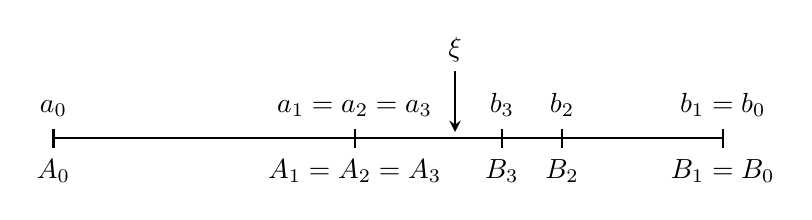
\begin{tikzpicture}[x=8.5cm, y=1cm]
    \draw[thick] (0,0) -- (1,0);
    
    % a0 / A0
    \draw[thick] (0, 0.12) -- (0, -0.12);
    \node[above] at (0, 0.15) {$a_0$};
    \node[below] at (0, -0.15) {$A_0$};

    % a1 = a2 = a3 / A1 = A2 = A3
    \draw[thick] (0.45, 0.12) -- (0.45, -0.12);
    \node[above] at (0.45, 0.15) {$a_1 = a_2 = a_3$};
    \node[below] at (0.45, -0.15) {$A_1 = A_2 = A_3$};

    % xi with arrow pointing down
    \draw[->, >=stealth, thick] (0.6, 0.85) -- (0.6, 0.08);
    \node[above] at (0.6, 0.85) {$\xi$};

    % b3 / B3
    \draw[thick] (0.67, 0.12) -- (0.67, -0.12);
    \node[above] at (0.67, 0.15) {$b_3$};
    \node[below] at (0.67, -0.15) {$B_3$};

    % b2 / B2
    \draw[thick] (0.76, 0.12) -- (0.76, -0.12);
    \node[above] at (0.76, 0.15) {$b_2$};
    \node[below] at (0.76, -0.15) {$B_2$};

    % b1 = b0 / B1 = B0
    \draw[thick] (1, 0.12) -- (1, -0.12);
    \node[above] at (1, 0.15) {$b_1 = b_0$};
    \node[below] at (1, -0.15) {$B_1 = B_0$};
\end{tikzpicture}
\end{center}

\begin{enumerate}[(i)]
    \item 我們將 $\overline{A_0 B_0}=[a_0, b_0]$ 等分為兩段，亦即 $[a_0, \frac{a_0+b_0}{2}]$ 和 $[\frac{a_0+b_0}{2}, b_0]$；而把 $\xi$ 所在的那一段叫做 $\overline{A_1 B_1}=[a_1, b_1]$（如果 $\xi = \frac{a_0+b_0}{2}$，就隨便取其中一段叫做 $\overline{A_1 B_1}=[a_1, b_1]$）. 換句話說，當 $a_0 \le \xi \le \frac{a_0+b_0}{2}$ 時，$a_1 = a_0,\; b_1 = \frac{a_0+b_0}{2}$. 當 $\frac{a_0+b_0}{2} \le \xi \le b_0$ 時，$a_1 = \frac{a_0+b_0}{2},\; b_1 = b_0$. 這樣逐次用二等分由 $\overline{A_1 B_1}$ 求得 $\overline{A_2 B_2}, \dots\dots$，由 $\overline{A_{n-1} B_{n-1}}$ 求得 $\overline{A_n B_n}$.
    \item 如此逐步用二分法縮小範圍，就得到
    \begin{align*}
    \overline{A_0 B_0} = [a_0, b_0] &\supseteq \overline{A_1 B_1} = [a_1, b_1] \supseteq \dots\dots \supseteq \overline{A_n B_n} \\
    &= [a_n, b_n] \supseteq \overline{A_{n+1} B_{n+1}} \\
    &= [a_{n+1}, b_{n+1}] \supseteq \dots\dots \supseteq \{\xi\}.
    \end{align*}
    而且
    \[
    \overline{A_n B_n} = \frac{1}{2}\overline{A_{n-1} B_{n-1}} = \frac{1}{4}\overline{A_{n-2} B_{n-2}} = \dots\dots = \frac{1}{2^n}\overline{A_0 B_0} = \frac{1}{2^n}(b_0 - a_0).
    \]
    也就是
    \[
    a_0 \le a_1 \le a_2 \le \cdots \le a_n \le \cdots \le \xi \le \cdots \le b_n \le \cdots \le b_2 \le b_1 \le b_0.
    \]
    而且 $b_n - a_n = \frac{1}{2}(b_{n-1}-a_{n-1}) = \dots\dots = \frac{1}{2^n}(b_0-a_0)$ 當 $n$ 趨於無窮時其極限為 0，故有
    \item[(iii)] $\langle a_n \rangle$ 是一個遞增數列，$\langle b_n \rangle$ 是一個遞減數列，皆以 $\xi$ 為極限，也就是
    \[
    \lim_{n\to\infty} a_n = \xi = \lim_{n\to\infty} b_n.
    \]
    （$\langle a_n \rangle, \langle b_n \rangle$ 分別自 $\xi$ 的「左方」及「右方」逼近 $\xi$.）
    \item[(iv)] 如果 $a_0, b_0$ 都是有理數的話，顯然 $a_n, b_n$ 也都是有理數. 所以這時 $\langle a_n \rangle, \langle b_n \rangle$ 都是有理數數列. 而 (iii) 式就相當於我們最初所要說明的“任何一實數都是某一適當有理數數列的極限”.
\end{enumerate}

\subsubsection*{2-3 $\sqrt{2}$ 的近似值：}

現在以 $\xi = \sqrt{2},\; a_0 = 1,\; b_0 = 2$ 為例，說明如何去求 $\sqrt{2}$ 的近似值.

\begin{center}
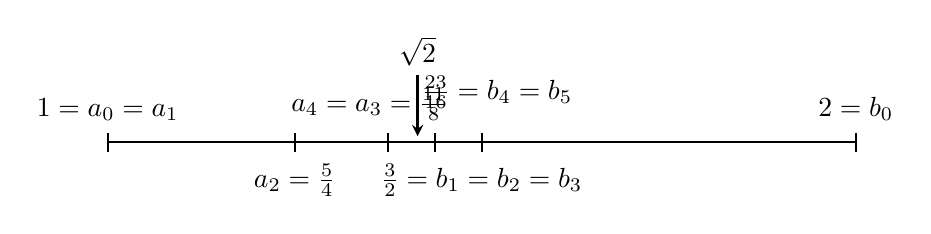
\begin{tikzpicture}[x=9.5cm, y=1cm]
    \draw[thick] (0, 0) -- (1, 0);
    
    % 1 = a0 = a1
    \draw[thick] (0, 0.12) -- (0, -0.12);
    \node[above] at (0, 0.15) {$1 = a_0 = a_1$};

    % a2 = 5/4 = 0.25
    \draw[thick] (0.25, 0.12) -- (0.25, -0.12);
    \node[below] at (0.25, -0.15) {$a_2 = \frac{5}{4}$};

    % a4 = a3 = 11/8 = 0.375
    \draw[thick] (0.375, 0.12) -- (0.375, -0.12);
    \node[above] at (0.35, 0.15) {$a_4 = a_3 = \frac{11}{8}$};

    % sqrt(2) arrow at 0.4142
    \draw[->, >=stealth, thick] (0.4142, 0.85) -- (0.4142, 0.08);
    \node[above] at (0.4142, 0.85) {$\sqrt{2}$};

    % 23/16 = b4 = b5 = 0.4375
    \draw[thick] (0.4375, 0.12) -- (0.4375, -0.12);
    \node[above] at (0.52, 0.3) {$\frac{23}{16} = b_4 = b_5$};

    % 3/2 = b1 = b2 = b3 = 0.5
    \draw[thick] (0.5, 0.12) -- (0.5, -0.12);
    \node[below] at (0.5, -0.15) {$\frac{3}{2} = b_1 = b_2 = b_3$};

    % 2 = b0
    \draw[thick] (1, 0.12) -- (1, -0.12);
    \node[above] at (1, 0.15) {$2 = b_0$};
\end{tikzpicture}
\end{center}

\begin{align}
\frac{1}{2}(a_0+b_0) = \frac{3}{2},&\quad \left(\frac{3}{2}\right)^2 = \frac{9}{4} > 2 \implies \frac{3}{2} > \sqrt{2}, \notag \\
\text{故}\quad a_1 = a_0 = 1,&\quad b_1 = \frac{3}{2}; \\
\frac{1}{2}(a_1+b_1) = \frac{5}{4},&\quad \left(\frac{5}{4}\right)^2 = \frac{25}{16} < 2 \implies \frac{5}{4} < \sqrt{2}, \notag \\
\text{故}\quad a_2 = \frac{5}{4},&\quad b_2 = b_1 = \frac{3}{2}; \\
\frac{1}{2}(a_2+b_2) = \frac{11}{8},&\quad \left(\frac{11}{8}\right)^2 = \frac{121}{64} < 2 \implies \frac{11}{8} < \sqrt{2}, \notag \\
\text{故}\quad a_3 = \frac{11}{8},&\quad b_3 = b_2 = \frac{3}{2}; \\
\frac{1}{2}(a_3+b_3) = \frac{23}{16},&\quad \left(\frac{23}{16}\right)^2 = \frac{529}{256} > 2 \implies \frac{23}{16} > \sqrt{2}, \notag \\
\text{故}\quad a_4 = a_3 = \frac{11}{8},&\quad b_4 = \frac{23}{16}; \\
\frac{1}{2}(a_4+b_4) = \frac{45}{32},&\quad \left(\frac{45}{32}\right)^2 = \frac{2025}{1024} < 2 \implies \frac{45}{32} < \sqrt{2}, \notag \\
\text{故}\quad a_5 = \frac{45}{32},&\quad b_5 = b_4 = \frac{23}{16}; \\
&\ \ \dots\dots\dots\dots\dots\dots\dots\dots \notag
\end{align}
如此逐步計算，每次只要檢驗「$\frac{1}{2}(a_{n-1}+b_{n-1})$ 的平方」和 2 之間的大小次序關係，就能確定 $\frac{1}{2}(a_{n-1}+b_{n-1})$ 應該是 $a_n$ 還是 $b_n$. 顯然的，這樣所求得的 $a_n, b_n$ 和 $\sqrt{2}$ 有下列關係：
\[
a_n < \sqrt{2} < b_n,\quad b_n - a_n = \frac{1}{2^n}.
\]
我們可以把 $a_n$ 叫做 $\sqrt{2}$ 的一個「$n$ 階左近似值」，$b_n$ 叫做 $\sqrt{2}$ 的一個「$n$ 階右近似值」；它們和 $\sqrt{2}$ 的差小於 $\frac{1}{2^n}$.

\subsection*{習題 3-2}

\begin{enumerate}
    \item 用二分逼近法求方程式 $x^3+x-3=0$ 在 1 與 2 之間的根的左右近似值，準確到 $1/2^5$.
    \item 利用下列不等式，寫出 $\sqrt{3}+\sqrt{2}, \sqrt{3}-\sqrt{2}, \sqrt{3}\cdot\sqrt{2}$ 的逼近數列的前四項：
    \begin{alignat*}{2}
    1.4 &< \sqrt{2} < 1.5, &\qquad 1.7 &< \sqrt{3} < 1.8, \\
    1.41 &< \sqrt{2} < 1.42, &\qquad 1.73 &< \sqrt{3} < 1.74, \\
    1.414 &< \sqrt{2} < 1.415, &\qquad 1.732 &< \sqrt{3} < 1.732, \\
    1.4142 &< \sqrt{2} < 1.4143, &\qquad 1.7320 &< \sqrt{3} < 1.7321.
    \end{alignat*}
    \item 用二分逼近法求下列數的左右近似值，準確到 $1/2^5$.
    \begin{enumerate}[(a)]
        \item $\sqrt[3]{2}$.
        \item $\sqrt{5}$.
        \item $\sqrt{7}$.
        \item $\sqrt{\frac{3}{5}}$.
    \end{enumerate}
\end{enumerate}

\subsection{實數系的完備性與實數系的基本性質}\label{sec:b2_3-3}

\subsubsection*{3-1 對於加乘及不等式運算，實數系和有理數系具有完全相同的性質；為便於同學們參考與引用，將它們列述如下：}

對於實數系中的任意元素 $a, b, c \in \mathbb{R}$，恆有
\begin{enumerate}
    \item[(I)] $(a+b)+c = a+(b+c)$; $(ab)c = a(bc)$. \hfill 〔結合律〕
    \item[(II)] $a+b = b+a$; $ab = ba$. \hfill 〔交換律〕
    \item[(III)] $a+0 = 0+a = a$; $a\cdot 0 = 0\cdot a = 0$. \hfill 〔零的特性〕
    \item[(IV)] $a\cdot 1 = 1\cdot a = a$. \hfill 〔1 的特性〕
    \item[(V)] 對於任意 $a$，存在有唯一的一 $-a$，使得 $a+(-a) = 0$；\\
    對於任意 $a\neq 0$，存在有唯一的一 $\frac{1}{a}$，使得
    \[
    a\cdot \frac{1}{a} = 1. \hfill \text{〔可逆性〕}
    \]
    \item[(VI)] $a(b+c) = ab+ac$. \hfill 〔分配律〕
    \item[(I$'$)] $a>b \iff b<a$.
    \item[(II$'$)] $a>b \text{ 和 } b>c \implies a>c$.
    \item[(III$'$)] 對於任意實數 $a, b$，下列關係中有一種且僅有一種成立：
    \[
    a>b,\quad a=b \quad \text{或 } a<b.
    \]
    \item[(IV$'$)] $a>b \implies a+c < b+c$.\phantomsection\label{note:b2-ch3-prop-iv-prime}
    \item[(V$'$)] $a>b \text{ 和 } c>d \implies a+c > b+d$.
    \item[(VI$'$)] $a>b \text{ 和 } c>0 \implies ac>bc$.
    \item[(VII$'$)] $a>b \text{ 和 } c<0 \implies ac<bc$.
    \item[(VIII$'$)] 對於任意兩個正實數 $a, b>0$，恆存在有一夠大的正整數 $n$，使得 $na>b$.（通稱之為阿基米德性質.）
\end{enumerate}

\paragraph{註：} 當年阿基米德提出這個實數的基本性質，想必是從龜兔賽跑這個耐人尋味的故事中領悟而來的. 玆有下圖為證：

\begin{center}
\begin{tikzpicture}[x=1cm, y=1cm, line cap=round, line join=round]
    % Top segment: turtle stride length a
    \draw[|-|, thick] (2.2, 5.0) -- (3.2, 5.0);
    \node[above] at (2.7, 5.0) {$a$};
    \node[right, font=\normalsize] at (3.3, 5.0) {：龜步步幅};

    % Speech bubble for tortoise
    \draw[thick, fill=white, rounded corners=4pt] (5.5, 2.7) rectangle (7.4, 4.7);
    \draw[thick] (6.4, 2.7) -- (5.7, 2.2) -- (6.1, 2.7);
    \node[align=center, font=\footnotesize] at (6.45, 3.7) {
        一萬、一萬零一$\cdots$\\
        阿基米德性質\\
        證起來真是\\
        累死我了！
    };

    % Start indicator
    \draw[->, >=stealth, very thick] (0.5, 2.5) -- (0.5, 1.4);
    \node[draw, thick, fill=white, font=\footnotesize, inner sep=2pt] at (0.5, 2.2) {起點};

    % Upper line (Tortoise track)
    \draw[very thick, ->] (-0.5, 1.3) -- (10.2, 1.3);
    \draw[thick] (0.5, 1.45) -- (0.5, 1.15);
    \node[below, font=\normalsize] at (0.5, 1.15) {$0$};
    
    % Ticks along the track
    \draw[thick, dashed] (1.8, 1.45) -- (2.6, 1.45);
    \draw[thick] (3.6, 1.45) -- (3.6, 1.15);
    \draw[thick] (4.6, 1.45) -- (4.6, 1.15);
    \draw[thick] (5.6, 1.45) -- (5.6, 1.15);
    \draw[thick] (6.6, 1.45) -- (6.6, 1.15);

    % Tortoise on upper line at around x=5.6
    \begin{scope}[shift={(5.6, 1.45)}, scale=0.6]
        % Shell
        \draw[thick, fill=gray!15] (-0.9, 0) arc (180:0:0.9cm and 0.55cm) -- cycle;
        % Scutes pattern
        \draw[thin] (-0.5, 0.45) -- (-0.2, 0);
        \draw[thin] (0.5, 0.45) -- (0.2, 0);
        \draw[thin] (0, 0.55) -- (0, 0);
        \draw[thin] (-0.7, 0.25) -- (0.7, 0.25);
        % Head & neck
        \draw[thick] (0.8, 0.1) arc (-60:70:0.35cm and 0.25cm) -- (1.1, 0.4) arc (70:-120:0.2cm) -- (0.85, 0.05);
        \fill (1.15, 0.38) circle (1pt);
        % Legs
        \draw[thick] (-0.7, 0) -- (-0.8, -0.2) -- (-0.6, -0.2);
        \draw[thick] (-0.3, 0) -- (-0.4, -0.2) -- (-0.2, -0.2);
        \draw[thick] (0.4, 0) -- (0.3, -0.2) -- (0.5, -0.2);
        \draw[thick] (0.7, 0) -- (0.8, -0.2) -- (1.0, -0.2);
        % Tail
        \draw[thick] (-0.9, 0.05) -- (-1.1, 0.0);
    \end{scope}

    % Lower line (Hare track)
    \draw[very thick, ->] (-0.5, 0) -- (10.2, 0);
    \draw[thick] (0.5, 0.15) -- (0.5, -0.15);
    \node[above, font=\normalsize] at (0.5, 0.15) {$0$};

    % Tick at b
    \draw[thick] (8.3, 0.15) -- (8.3, -0.15);
    \node[below, font=\normalsize] at (8.3, -0.15) {$b$};

    % Sleeping Hare at position b
    \begin{scope}[shift={(8.3, 0.25)}, scale=0.65]
        % Body
        \draw[thick, fill=white] (-0.8, 0) arc (180:20:0.8cm and 0.5cm) arc (20:-160:0.8cm and 0.3cm) -- cycle;
        % Head
        \draw[thick, fill=white] (-0.6, 0.2) circle (0.3cm);
        % Closed eye
        \draw[thick] (-0.7, 0.2) arc (180:360:0.1cm and 0.05cm);
        % Ears lying back
        \draw[thick] (-0.4, 0.4) .. controls (0.2, 0.8) .. (0.7, 0.5) .. controls (0.2, 0.4) .. (-0.3, 0.3);
        \draw[thick] (-0.5, 0.45) .. controls (0.1, 0.95) .. (0.8, 0.7) .. controls (0.3, 0.55) .. (-0.4, 0.35);
        % Paws & Tail
        \draw[thick] (0.7, 0.1) arc (-30:150:0.2cm and 0.15cm);
        \draw[thick] (-0.2, -0.15) arc (0:180:0.2cm and 0.1cm);
    \end{scope}

    % Snoring Zzz
    \node[font=\footnotesize] at (7.6, 0.55) {$z$};
    \node[font=\small] at (7.4, 0.8) {$z$};
    \node[font=\normalsize] at (7.6, 1.05) {$Z$};
\end{tikzpicture}
\end{center}

\subsubsection*{3-2 實數系的完備性：}

由上節所述，我們看出實數系與有理數系在加、乘及不等式的運算有完全相同的性質. 但是實數系與有理數系在極限方面卻有很重大的差異. 譬如在上一節中我們所求得的兩個有理數數列 $\langle a_n \rangle, \langle b_n \rangle$.
\begin{gather*}
1 = a_0 \le a_1 \le a_2 \le \cdots \le a_n \le \cdots \le \sqrt{2} \le \cdots \le b_n \le \cdots \le b_2 \le b_1 \le b_0 = 2, \\
\lim_{n\to\infty}(b_n-a_n) = \lim_{n\to\infty}\frac{1}{2^n} = 0.
\end{gather*}
它們的極限 $\sqrt{2}$ 卻不是有理數，也就是說
\[
a_n, b_n \in \mathbb{Q};\quad \text{但是 } \lim_{n\to\infty} a_n = \sqrt{2} = \lim_{n\to\infty} b_n \notin \mathbb{Q}.
\]
換句話說，一個完全由有理數所組成的數列，它的極限不一定是有理數. 所以對於極限來說，有理數系顯然不夠完備. 但是相反的實數系對於極限來說是完備的. 實數系的完備性可以敘述成好幾種不同的形式. 我們在這裡先敘述下面兩種形式：

(IX$'$) 完備性（第一形式）：設 $\langle a_n \rangle, \langle b_n \rangle$ 是兩個實數數列滿足下列性質：
\begin{enumerate}[(i)]
    \item $a_1 \le a_2 \le \dots\dots \le a_n \le \dots\dots \le b_n \le \dots\dots \le b_2 \le b_1$,
    \item $\lim_{n\to\infty}(b_n-a_n) = 0$.
\end{enumerate}
就必定存在有一個實數 $\xi$，使得
\[
\lim_{n\to\infty} a_n = \xi = \lim_{n\to\infty} b_n.
\]
完備性（第二形式）：如果 $\langle a_n \rangle$ 是一個有上界 $c$ 的遞增數列，$a_1 \le a_2 \le \dots\dots \le c$. 就會有一個實數 $\xi$，使得
\[
\lim_{n\to\infty} a_n = \xi \le c.
\]
上述完備性 (IX$'$) 和前述性質 (I)$\sim$(VI), (I$'$$\sim$(VIII$'$) 就構成實數系的一組基本性質. 所有其他的實數系性質都是它們的邏輯推論.

我們在這裡再強調一次；實數系與有理數系間最基本的差異，便在於上述的完備性. 事實上，實數系的完備性乃是微積分學的基礎. 由於同學們目前所知有限，在現階段無法對此深切體會. 不過我們將以下列定理為例，來說明完備性的一個應用.

\subsection*{習題 3-3}

\begin{enumerate}
    \item 證明任意兩實數 $a, b$ 之間，一定存在有理數 $c$，使得 $a < c < b$（用阿基米德性質）
    \item 利用實數的完備性，證明下列敘述：\\
    設 $\langle a_n \rangle$ 是一個遞減數列，並且有一個下界 $c$，（即 $c < a_n\; \forall n$），則數列 $\langle a_n \rangle$ 的極限存在，而且 $c \le \lim_{n\to\infty} a_n$.
    \item 如果 $a>0$，證明數列 $a_1 = a, a_2 = 2a, \dots\dots a_n = na \dots\dots$ 沒有上限. 由此證明阿基米德性質：$a>0, b$ 任意實數，則存在正整數 $n$，使得 $nc > d$\phantomsection\label{note:b2-ch3-ex3-3-q3-nc-d}.
    \item 設 $a, b$ 是兩個正實數，證明：
    \begin{enumerate}[(i)]
        \item 如果 $a>b$，則 $\lim_{n\to\infty}\left(\frac{a}{b}\right)^n = \infty$.
        \item 如果 $a<b$，則 $\lim_{n\to\infty}\left(\frac{a}{b}\right)^n = 0$.
    \end{enumerate}
    \item 設 $a, b$ 是兩個正實數，而且 $a>1$，利用阿基米德性質，證明存在自然數 $n$，使 $a^n > b$ 成立.
    \item 設 $n$ 是自然數，$a$ 是實數，證明
    \[
    (1+a)^n \ge 1+na.
    \]
    \item 如果 $P$ 是質數，$P>0$，證明 $\sqrt{P}$ 是無理數.
    \item 設 $\alpha, \beta, \gamma$ 是三個正實數，
    \begin{enumerate}[(i)]
        \item 如果 $\alpha < \beta$，證明 $\frac{\alpha}{1+\alpha} < \frac{\beta}{1+\beta}$.
        \item 如果 $\alpha+\beta = \gamma$，證明 $\frac{\gamma}{1+\gamma} < \frac{\alpha}{1+\alpha} + \frac{\beta}{1+\beta}$.
    \end{enumerate}
\end{enumerate}

\subsection{中間值定理}\label{sec:b2_3-4}

下述定理是實數系完備性的一個重要推論.

\begin{theorem}[多項式函數的中間值定理]
設 $f(x)$ 是一個實係數多項式，而 $a, b$ 為兩個給定實數，且 $a < b$. 如果 $f(a)$ 和 $f(b)$ 異號，那麼在 $a, b$ 之間一定至少有一個 $f(x)=0$ 的根.（至少有一個實數 $\xi, a < \xi < b$ 而且 $f(\xi)=0$.）
\end{theorem}

如果我們畫一個圖

\begin{center}
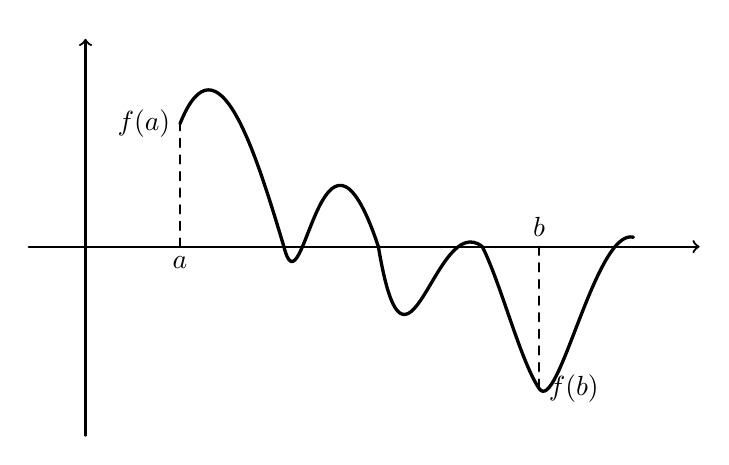
\begin{tikzpicture}[x=1.2cm, y=1.2cm, line cap=round, line join=round]
    % Axes
    \draw[thick, ->] (-0.6, 0) -- (6.5, 0);
    \draw[thick, ->] (0, -2.0) -- (0, 2.2);

    % Curve crossing x-axis multiple times between a and b
    % Let a = 1.0, b = 4.8
    \coordinate (A) at (1.0, 1.3);
    \coordinate (B) at (4.8, -1.5);

    \draw[very thick] (1.0, 1.3) .. controls (1.4, 2.3) and (1.8, 1.0) .. (2.1, 0)
                                .. controls (2.3, -0.8) and (2.5, 1.8) .. (3.1, 0)
                                .. controls (3.4, -1.8) and (3.7, 0.4) .. (4.2, 0)
                                .. controls (4.4, -0.4) and (4.6, -1.2) .. (4.8, -1.5)
                                .. controls (5.0, -1.8) and (5.4, 0.2) .. (5.8, 0.1);

    % Dashed vertical lines at a and b
    \draw[dashed, thick] (1.0, 0) -- (A);
    \draw[dashed, thick] (4.8, 0) -- (B);

    % Points and labels
    \node[below, font=\normalsize] at (1.0, 0) {$a$};
    \node[left, font=\normalsize] at (A) {$f(a)$};
    \node[above, font=\normalsize] at (4.8, 0) {$b$};
    \node[right, font=\normalsize] at (B) {$f(b)$};
\end{tikzpicture}
\end{center}

那麼定理 1，在直觀上是顯而易見的.

\noindent\textbf{【證明】}
顯然我們只需要討論 $f(a)>0, f(b)<0$ 的情形，因為對於 $f(a)<0, f(b)>0$ 的情形，我們只要改為討論 $-f(x)$ 就可以了. 現在取 $a_0 = a, b_0 = b$，利用 § 2 中的二分法討論如下：
\[
\begin{cases}
\text{如果 } f\left(\frac{a_0+b_0}{2}\right) = 0, & \text{則定理 1 已經成立了，不必再多作討論.} \\[1em]
\text{如果 } f\left(\frac{a_0+b_0}{2}\right) > 0, & \text{就取 } a_1 = \frac{a_0+b_0}{2},\; b_1 = b_0. \\[1em]
\text{如果 } f\left(\frac{a_0+b_0}{2}\right) < 0, & \text{就取 } a_1 = a_0,\; b_1 = \frac{a_0+b_0}{2}.
\end{cases}
\]

\begin{center}
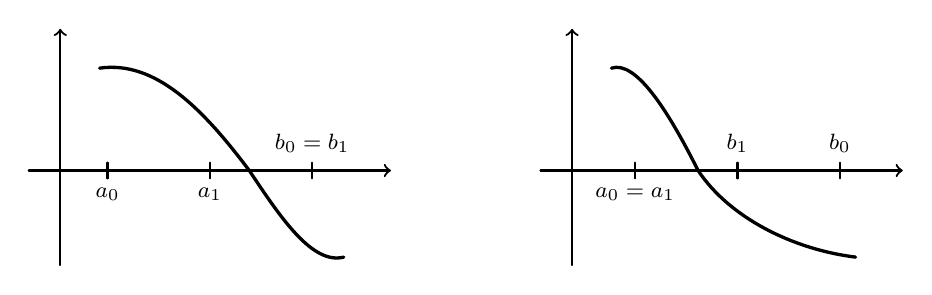
\begin{tikzpicture}[scale=1.0, line cap=round, line join=round]
    % Diagram 1: f((a0+b0)/2) > 0
    \begin{scope}[xshift=0cm]
        \draw[thick, ->] (-0.4, 0) -- (4.2, 0);
        \draw[thick, ->] (0, -1.2) -- (0, 1.8);
        
        % Curve
        \draw[very thick] (0.5, 1.3) .. controls (1.2, 1.4) and (1.8, 0.8) .. (2.4, 0)
                                    .. controls (2.8, -0.6) and (3.2, -1.2) .. (3.6, -1.1);

        \draw[thick] (0.6, 0.1) -- (0.6, -0.1);
        \node[below, font=\footnotesize] at (0.6, -0.1) {$a_0$};

        \draw[thick] (1.9, 0.1) -- (1.9, -0.1);
        \node[below, font=\footnotesize] at (1.9, -0.1) {$a_1$};

        \draw[thick] (3.2, 0.1) -- (3.2, -0.1);
        \node[above, font=\footnotesize] at (3.2, 0.1) {$b_0 = b_1$};
    \end{scope}

    % Diagram 2: f((a0+b0)/2) < 0
    \begin{scope}[xshift=6.5cm]
        \draw[thick, ->] (-0.4, 0) -- (4.2, 0);
        \draw[thick, ->] (0, -1.2) -- (0, 1.8);
        
        % Curve
        \draw[very thick] (0.5, 1.3) .. controls (0.8, 1.4) and (1.2, 0.8) .. (1.6, 0)
                                    .. controls (2.0, -0.6) and (2.8, -1.0) .. (3.6, -1.1);

        \draw[thick] (0.8, 0.1) -- (0.8, -0.1);
        \node[below, font=\footnotesize] at (0.8, -0.1) {$a_0 = a_1$};

        \draw[thick] (2.1, 0.1) -- (2.1, -0.1);
        \node[above, font=\footnotesize] at (2.1, 0.1) {$b_1$};

        \draw[thick] (3.4, 0.1) -- (3.4, -0.1);
        \node[above, font=\footnotesize] at (3.4, 0.1) {$b_0$};
    \end{scope}
\end{tikzpicture}
\end{center}

總之，除了 $f\left(\frac{a_0+b_0}{2}\right) = 0$ 這個顯然成立的情形以外，我們可以用二分法從 $[a_0, b_0]$ 中選得半段 $[a_1, b_1]$ 依然保有 $f(a_1)>0, f(b_1)<0$ 這個原來的假設條件. 所以我們又可以同樣地用二分法從 $[a_1, b_1]$ 求得 $[a_2, b_2]$，並且依然保有 $f(a_2)>0, f(b_2)<0$ 這個原始條件.

如此逐次二等分，假如在某一次的等分點 $\frac{a_n+b_n}{2}$ 滿足 $f\left(\frac{a_n+b_n}{2}\right) = 0$，則定理 1 就成立了，也不必再多作討論. 假如對每一次的等分點 $\frac{a_n+b_n}{2}$，$f\left(\frac{a_n+b_n}{2}\right)$ 都不是 0，那麼可以按上述二分法繼續不斷的進行，就能得到滿足下列性質的數列 $\langle a_n \rangle$ 和 $\langle b_n \rangle$：
\begin{enumerate}[(i)]
    \item $f(a_n)>0, f(b_n)<0, n=1, 2, 3, \dots\dots$
    \item $a = a_0 \le a_1 \le a_2 \le \dots\dots \le a_n \le \dots\dots \le b_n \le \dots\dots \le b_2 \le b_1 \le b_0$.
    \item $\lim_{n\to\infty}(b_n-a_n) = \lim_{n\to\infty}\frac{b-a}{2^n} = 0$.
\end{enumerate}
由實數的完備性及 (ii), (iii) 得知存在一個實數 $\xi$，
\[
\lim_{n\to\infty} a_n = \xi = \lim_{n\to\infty} b_n
\]
又由 (i) 知道
\[
\lim_{n\to\infty} f(a_n) \ge 0 \quad \text{和} \quad \lim_{n\to\infty} (b_n) \le 0\phantomsection\label{note:b2-ch3-lim-bn}.
\]
因為 $f(x)$ 是多項式，由極限的四則運算可以得到：
\begin{align*}
\lim_{n\to\infty} f(a_n) &= f(\lim_{n\to\infty} a_n) = f(\xi) \ge 0, \\
\lim_{n\to\infty} f(b_n) &= f(\lim_{n\to\infty} b_n) = f(\xi) \le 0.
\end{align*}
因為 $f(\xi)\ge 0$ 和 $f(\xi)\le 0$ 需要同時成立，所以 $f(\xi)=0$.
\hfill（定理 1 證畢）

\paragraph{【例 1】} $f(x) = 2x^2+7x+1$ \\
因 $f(0) = 1 > 0$ 及 $f(-1) = -4 < 0$，\\
所以 $f(x)=0$ 在 $[-1, 0]$ 之間有一實根. \\
又因 $f(-3) = -2 < 0$ 及 $f(-4) = 5 > 0$，\\
所以 $f(x)=0$ 在 $[-4, -3]$ 之間也有一實根.

\begin{prop}[推論]
設 $a$ 是一個正實數，$n$ 是一個正整數，那麼就有一個唯一的正實數 $\xi$，使得 $\xi^n = a$.（我們因而用 $\sqrt[n]{a}$ 表示滿足 $x^n = a$ 的唯一正實數 $\xi$.）
\end{prop}

\noindent\textbf{【證明】} 令 $f(x) = x^n - a,\; b = a+1$. 顯然有
\begin{align*}
f(0) &= -a < 0, \\
f(b) &= (1+a)^n - a \ge 1+(n-1)a > 0,
\end{align*}
由定理 1 得知 $[0, b]$ 之間至少有 $f(x)=0$ 的一個實根.

現在我們再證唯一性；設 $\xi_1, \xi_2$ 是兩個滿足 $f(x)=0$ 的正實數：
\[
\xi_1^n - a = 0,\quad \xi_2^n - a = 0.
\]
兩式相減，得到
\[
\xi_1^n - \xi_2^n = 0,\quad \text{亦即 } \xi_1^n = \xi_2^n.
\]
所以 $\xi_1$ 必定和 $\xi_2$ 相同，要不然的話，由性質 (III$'$) 有
\[
\xi_1 > \xi_2,\quad \text{或 } \xi_1 < \xi_2.
\]
但是
\begin{align*}
\xi_1 > \xi_2 > 0 &\implies \xi_1^n > \xi_2^n > 0, \\
0 < \xi_1 < \xi_2 &\implies 0 < \xi_1^n < \xi_2^n.
\end{align*}
這顯然和 $\xi_1^n = \xi_2^n$ 相矛盾. 換句話說，$\xi_1 \neq \xi_2$ 是不可能的，所以只好 $\xi_1 = \xi_2$. 但是 $\xi_1, \xi_2$ 是 $f(x)=0$ 的任意正根，故 $f(x)=0$ 的正根只有一個.

定理 1 的另外一個重要推論可寫成：

\begin{theorem}
$f(x)$ 是一個奇數次實係數多項式，那麼方程式 $f(x)=0$ 至少有一實根.
\end{theorem}

\noindent\textbf{【證明】} 基於定理 1，我們只要能求得兩個實數 $\alpha, \beta$，使得奇數次多項式 $f(x)$ 在 $\alpha, \beta$ 的值異號.（即 $f(\alpha)f(\beta)<0$ 就可以了.）當然我們還可以假設 $f(x)$ 的首項係數是正的，要不然我們只要把 $f(x)$ 換成 $-f(x)$ 來討論就行了.

設 $f(x) = a_n x^n + a_{n-1} x^{n-1} + \dots\dots + a_0,\; a_n > 0,\; n$ 為奇數，我們希望找到一個大的正數 $k$，使得
\[
a_n k^n > |a_{n-1} k^{n-1} + \dots\dots + a_0|.
\]
那麼，
\begin{align*}
f(k) &= a_n k^n + a_{n-1} k^{n-1} + \dots\dots + a_0 \\
&\ge a_n k^n - |a_{n-1} k^{n-1} + \dots\dots + a_0| \\
&\ge 0.
\end{align*}
另一方面，
\begin{align*}
f(-k) &= a_n (-k)^n + a_{n-1} (-k)^{n-1} + \dots\dots + a_0 \\
&= -[(a_n k^n) - (a_{n-1} (-k)^{n-1} + \dots\dots + a_0)] \\
&\le -(a_n k^n - |a_{n-1} k^{n-1} + \dots\dots + a_0|) \\
&< 0.
\end{align*}
那麼就可以運用定理 1 而得到一個實根了.

現在的問題就是如何找到這樣一個 $k$，我們知道對於任一實數 $k > 1$，且 $m = \operatorname{Max}(|a_{n-1}|, \dots\dots, |a_0|)$，則
\begin{align*}
|a_{n-1} k^{n-1} + \dots\dots + a_0| &\le |a_{n-1} k^{n-1}| + \dots\dots + |a_0| \\
&\le n m k^{n-1}
\end{align*}
比較 $a_n k^n$ 與 $n m k^{n-1}$，我們知道如果取一個正整數 $k$ 滿足 $k a_n > n m$，那麼 $a_n k^n > n m k^{n-1}$ 當然成立. 也就是說 $a_n k^n > n m k^{n-1} \ge |a_{n-1} k^{n-1} + \dots\dots + a_0|$. 總括以上解析可知，只要按照阿基米德性質取一個正整數 $k$，使得 $k a_n > n m$，就有
\begin{align*}
f(k) &> 0 \\
f(-k) &< 0
\end{align*}
這個定理也就得證了.

\paragraph{【例 2】}
\begin{enumerate}[(i)]
    \item $x^5+10x^2+3=0$ 至少有一個負實根.
    \item $x^7+6x^4-1=0$ 至少有一個正實根.
\end{enumerate}

\paragraph{注意：} 定理 2 中 $n$ 是奇數是一個不可缺少的條件，譬如 $x^2+1=0$ 就顯然沒有實根. 因為對於任何實數 $a, a^2 \ge 0$，故有
\[
f(a) = a^2+1 \ge 1 \ge 0.
\]

\subsection*{習題 3-4}

\begin{enumerate}
    \item 找出下列各多項式方程式的所有實根的位置（在那兩個相鄰整數之間）：
    \begin{enumerate}[(i)]
        \item $x^4-10x^2+1=0$.（有四實根）
        \item $x^3-3x^2+3x-4=0$.（有一實根）
        \item $2x^5-5x^4-7x^3+16x^2+3x-3=0$.（有五實根）
    \end{enumerate}
    \item 設 $f(x)$ 是一個多項式，$a, b$ 是兩個實根\phantomsection\label{note:b2-ch3-ex3-4-q2-roots}，$a < b$. 如果實數 $c$ 在 $f(a)$ 與 $f(b)$ 之間（例如 $f(a) < c < f(b)$），證明存在實數 $\xi, a < \xi < b$，使得 $f(\xi) = c$.
    \item 如果在實係數多項式 $f(x) = a_0 + a_1 x + \dots\dots + a_n x^n$ 中 $a_0$ 與 $a_n$ 異號（即 $a_0 a_n < 0$），證明 $f(x)=0$ 必有一正實根.
    \item 下列方程式各有一個正實數根，利用多項式函數的中間值定理，求它們的近似值至三位小數：
    \begin{enumerate}[(i)]
        \item $x^2-5=0$.
        \item $x^2-4x-3=0$.
        \item $x^3-4=0$.
        \item $x^3-9x-10=0$.
    \end{enumerate}
    \item 設函數 $y=f(x)=3x^3-1$，利用多項式函數的中間值定理，證明在 0 與 1 之間有一個實數 $a$，使 $f(a)=a$ 成立.
\end{enumerate}

\subsection{連續函數}\label{sec:b2_3-5}

在證明多項式的中間值定理時，我們用到了兩個主要條件，一個就是實數的完備性，還有一個就是多項式函數的連續性，所謂連續性就是對於任意數列 $\langle a_n \rangle, a_n \to \xi$，我們有
\begin{equation}
\lim_{n\to\infty} f(a_n) = f(\lim_{n\to\infty} a_n) = f(\xi) \dots\dots\dots\dots\dots\dots (1)
\end{equation}
的關係. 因此可以推問，對於一般滿足條件 (1) 的函數，中間值定理也成立嗎？為了討論這個問題，我們把這類函數叫做連續函數，本節就是要討論連續函數的中間值定理.

\begin{definition*}[定義]
設 $f: A \longrightarrow B$ 是一個函數，而 $\xi$ 是 $A$ 中的一點，如果對於 $A$ 中的任意數列 $\langle a_n \rangle, a_n \to \xi$，我們有 $\lim_{n\to\infty} f(a_n) = f(\xi)$ 的話，就說函數 $f$ 在 $\xi$ 點連續. 如果 $f$ 在 $A$ 中每一點都連續，就說 $f$ 是 $A$ 上的一個連續函數，或簡稱為連續函數.
\end{definition*}

譬如多項式函數是連續函數. 又如 $y = [x]$（$[\ ]$ 是高斯符號，表示小於或等於 $x$ 的最大整數，見第一冊第五章）是從實數到整數的一個函數，它在整數點不連續，在其他的點都連續. 當然，不連續函數的例子還有很多，但在高中階段，我們用不著深究.

讓我們現在來考慮一個任意的連續函數 $f: A \longrightarrow B$，如果 $\xi$ 是 $A$ 中的一點，$\langle a_n \rangle, \langle b_n \rangle$ 是兩個趨近於 $\xi$ 的數列，而且
\[
b_1 \le b_2 \le \dots\dots \le b_n \le \dots\dots \le \xi \le \dots\dots \le a_n \le \dots\dots \le a_2 \le a_1.
\]
那麼由連續的定義，可以知道
\[
\lim_{n\to\infty} f(a_n) = \lim_{n\to\infty} f(b_n) = f(\xi).
\]
反過來我們還可以證明這也是連續函數的充分條件：\\
假設 $f: A \longrightarrow B$ 是一個函數，而 $\xi$ 是 $A$ 中的一點，如果對任意以 $\xi$ 為極限的遞減或遞增的數列 $\langle a_n \rangle$，都有 $\lim_{n\to\infty} f(a_n) = f(\xi)$，那麼函數 $f$ 在 $\xi$ 點連續.（因為證明複雜，在此略去不談）

\begin{theorem}[定理 $1'$（連續函數的中間值定理）]
設 $f(x)$ 是一個連續函數，而 $a, b$ 是兩個實數且 $a < b$. 如果 $f(a)$ 和 $f(b)$ 異號，那麼在 $a, b$ 之間一定有一個 $f(x)=0$ 的根（即有一實數 $\xi, a < \xi < b$ 而且 $f(\xi)=0$）.
\end{theorem}
因為證明幾乎與定理 1 完全一樣，所以我們不在此贅述了.

\begin{prop}[推論]
設 $f(x)$ 是一個連續函數，$a, b$ 是兩個實數，而且 $a < b$，$f(a) \neq f(b)$. 那麼對於任意一個介於 $f(a), f(b)$ 之間的數 $M$，一定有一個 $a, b$ 之間的實數 $\xi$，使得 $f(\xi)=M$.
\end{prop}

\noindent\textbf{【證明】}
我們不妨假設 $f(a) < f(b)$.（因為 $f(a) > f(b)$ 時，可以同樣處理）. 那麼 $M$ 滿足 $f(a) < M < f(b)$，如果考慮一個新的函數 $g$：
\[
g(x) = f(x) - M.
\]
那麼
\[
g(a) = f(a) - M < 0,\quad g(b) = f(b) - M > 0.
\]
因此根據定理 $1'$，一定有一實數 $\xi, a < \xi < b$，使得 $g(\xi)=0$. 換句話說
\[
f(\xi)-M = 0 \quad \text{或} \quad f(\xi)=M.
\]

\subsection*{習題 3-5}

\begin{enumerate}
    \item 設函數 $y = f(x) = \frac{x^2+1}{2x-1}$，則 $f(0) = -1, f(1) = 2$ 符號相反，討論方程式 $f(x)=0$ 在 $0 \le x \le 1$ 中是否有解？
    \item 證明下列各函數是連續，並利用連續函數的中間值定理求根的位置（介於那兩個相接的整數之間）.
    \begin{enumerate}[(i)]
        \item $y = f(x) = x|x| - \frac{1}{2}$.
        \item $y = f(x) = |x+1| - |x - \frac{2}{3}|$.
    \end{enumerate}
    \item 下列函數各在那些點不連續？
    \begin{enumerate}[(i)]
        \item $y = f(x) = [x^2+1]$.
        \item $y = f(x) = |x|$.
        \item $y = f(x) = [\frac{x+1}{2}]x + 1$.
        \item $y = f(x) = x\cdot |x|$.
    \end{enumerate}
    \item 討論下列有理函數，各在那些點連續？
    \begin{enumerate}[(i)]
        \item $y = f(x) = \frac{x+2}{x^2-1}$.
        \item $y = f(x) = \frac{x-1}{x^2+1}$.
        \item $y = f(x) = \frac{1}{x} + \frac{1}{x+1} + \frac{1}{x-1}$.
    \end{enumerate}
    \item 證明 (i) $y = f(x) = \frac{1}{x}$，除了 $x = 0$ 以外連續. \\
    (ii) $y = f(x) = \frac{1}{ax+b},\; a\neq 0$，除了 $x = \frac{b}{a}$ 外連續\phantomsection\label{note:b2-ch3-ex3-5-q5-sign}.
    \item 證明多項式函數都是連續函數.
\end{enumerate}
